\title{CSCI 4502 Progress Report}
\author{Dimitrios Economou\\Josh Weaver\\Thomas Horn}
\date{\today}

\documentclass[letterpaper]{article}
\usepackage{amsmath,amsthm,amscd,amssymb,tikz,leftidx,hyperref,enumitem,natbib,seqsplit}

\numberwithin{equation}{subsection}

\newcommand{\marg}[1]{\normalsize{{\footnote{{#1}}}}{\marginpar[\hfill\tiny\thefootnote$\rightarrow$]{{$\leftarrow$\tiny\thefootnote}}}}
\newcommand{\N}{\mathbb{N}}

\begin{document}
\maketitle

\section{Abstract}
Reddit is a large and rapidly growing social news and content aggregation Web site. In fact, Reddit has evolved from the front page of the internet to a self-contained community with a lot of internal discussions about various subjects\cite{Singer}. On Reddit, users submit content which can be external links or text posts to various areas of interest or topics called \emph{subreddits}. In general, we will attempt to cluster subreddits using different metrics and clustering methods. Clustering subreddits could be potentially useful for a subreddit recommender system, but out project is mainly an exploration of clustering subreddits in different ways. In particular, we will cluster subreddits based on how topically diverse their comment threads are. Weninger et al.\cite{weninger} used topic modeling to show that comment threads on Reddit form topical hierarchies. It would be interesting to carry out a similar analysis to explore topical differences between subreddits or types of subreddits. For example, discussion-based subreddits may be more topically diverse than image-based subreddits.

\section{Dataset}
Thanks to \textbackslash u \textbackslash Stuck\_in\_the\_Matrix of redditanalytics, we have access to all of the submission objects on Reddit and about five months worth of comment data (from September 2014 through January 2015). Since we will probably only use the comment data, we will focus on describing that. The data is organized into five files where each line is a JSON object representing a single comment. The fields of each JSON object are (among other things) the number of upvotes and downvotes (and the difference representing a score), the author, the subreddit, the creation time, the link or text if it is a self-post, and its parent comment id. In total, the dataset of five months of comments is 113.4 GB.

\subsection{Cleaning the data}
There are several fields in the comment JSON objects that we are not interested in, so we have gone through the dataset and removed these fields.

To get started, we decided to restrict the dataset to 645 popular subreddits. The list of subreddits and a subjective analysis of whether they are discussion-based (self), have a high, medium, or low density of link submissions, or are image-based (imgur) was done by Siege Media\cite{siege}. We removed all the comments not posted in one of these subreddits and added in a field to describe what type of subreddit they fall under. We can potentially use this new field as a class label.

Further, there are many comments which were posted but were deleted by the author or some other reason. We removed these comments as we need the comment bodies for our analyses.

\subsection{Basic facts about the data}
We will now describe some basic statistical facts about the test dataset, which is a reduction of one of the months of comment data and is what we are first running our algorithms on. Statistical facts about the bigger dataset will be given in the final report.

\begin{tabular}{l*{6}{l}r}
    Stat              & Comments per thread & Comments per subreddit \\
    \hline
    Count            & 82727    & 373 \\
    Mean             & 12       & 2681 \\
    Std              & 53       & 7921 \\
    Min              & 1        & 1 \\
    $Q_1$            & 1        & 122 \\
    $Q_2$            & 4        & 489 \\
    $Q_3$            & 9        & 1578 \\
    Max              & 4681     & 80523 \\
\end{tabular}

\section{Progress}
We have written scripts to clean the data and used them. We have done basic statistical analyses of the data to get to know it better. We have attempted clustering subreddits based on where users comment using hierarchical clustering.

We have written scripts to process the comment bodies. This process involves breaking the comments up into words, obtaining their stems, removing stopwords, removing non-words, counting unique words (actually stems), removing words that appear only once in any given subreddit, etc. We made extensive use of Python's Natural Language Toolkit (NLTK) to do this. We have spent a lot of time manipulating the data and putting it into different formats, including putting it in a SQLite database. However, we have not really needed to use the database yet.

After processing the comments, we have clustered subreddits based on words most frequently found in them. We have tried k-means clustering using cosine similarity. The results have been promising. Using k-means with 15 clusters yields some intuitive clusters. For example, we have (clusters are labeled with integers and these integers are not important)
\text{}\\

2:    bikebuilders, triathlon, motorcycles, cyclocross, adventures, bmx, bicycletouring, cycling, bicycling

3:    pcgaming, boardgames, gamedev, gamernews, gaming, vita, patientgamers, truegaming, pcmasterrace, iosgaming, gamingsuggestions, snes, retrogaming, gamingnews, xbox, xboxone, xbox360, zelda

4:    microsoft, dotnet, technews, design\_critiques, graphic\_design, programminghorror, learnprogramming, netsec, css, kickstarter, oculus, photoshop, programming, coding, androiddev, learnpython, geek, javascript, linux, java, web\_design, androidapps, softwaregore, technology, software, learnjavascript, webdev, tech

7:    ramen, cheesemaking, fromscratch, budgetfood, food, 52weeksofcooking, recipes, nutrition, slowcooking, grilling, steak, cookingforbeginners, foodhacks, tonightsdinner, smoking, fitmeals, spicy, eatsandwiches

8:    techsupport, computers, gamingpc, windows8, sysadmin, homelab, usenet, buildapc, retrobattlestations, hardware, talesfromtechsupport, 24hoursupport, htpc, applehelp, networking

9:    financialindependence, freelance, woweconomy, investing, personalfinance, advertising, tax, digitalnomad, portfolios, economy, hwstartups, socialmedia, finance, smallbusiness, austrian\_economics, bigseo, wallstreetbets, startups, business, marketing

11:    movies, scifi, dvdcollection, bestofnetflix, southpark

12:    winemaking, beertrade, wine, cider, mead, alcohol, retailporn, bourbon, cocktails, beer, beerporn,
\text{}\\

\noindent but we also have clusters such as
\text{}\\

10:    askphilosophy, businessschool, premed, geology, expats, science, nursing, askscience, emergencymedicine, cogsci, energy, acting, medicine, math, careerguidance, learnspanish, resumes, gradadmissions, computervision, motivation, vfx, chemistry, languagelearning, architecture, academiceconomics, college, artificial, medicalschool, latin, jobs, cscareerquestions, pharmacy, theydidthemath, compsci, physicaltherapy, consulting, statistics, russian, engineering, education, findapath, linguistics, neuroscience,
\text{}\\

\noindent which doesn't make much sense. Specifying more clusters, however, yields some more structure such as the cluster
\text{}\\

3:    learn\_arabic, learnspanish, languagelearning, latin, learndutch, italianlearning, russian, linguistics.
\text{}\\

It also refines the clusters further into clusters such as
\text{}\\

6:    vegan, vegetarian

15:    winemaking, wine, cider, mead.
\text{}\\

It is exciting to see such structure revealed from a simple clustering algorithm.

Figure ~\ref{fig:fig1} shows a (relevant) small portion (the actual plot is too big to show for the report) of a dendrogram obtained by hierarchical clustering using Ward's method.

\begin{figure}[h!]
    \label{fig:fig1}
  \caption{Hierarchical clustering of subreddits using a td-idf matrix (from test data), cosine similarity, and Ward's method.}
  \centering
  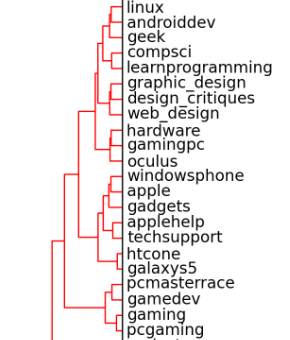
\includegraphics[width=0.5\textwidth]{sample1}
\end{figure}

\section{Problems}
A 113.4 GB dataset is a much larger dataset than any other dataset we have worked with. This indroduces many time- and memory-related issues. It takes a large time to clean the data and process the comments. Although performing more subtle language processing on the comment bodies yields better results, this substantially increases the computational complexity of our analyses. Even doing a relatively straightforward processing of the comment bodies takes a long time. We have also needed to learn about natural language processing in general, as well as topic modeling. For topic modeling, it is not practical to set up a database to do the work we want to do. So we have been relying on loading our data into memory for computing. We are therefore constrained by how much memory we can access.

Many clustering algorithms (such as k-means) requires the number of clusters to be specified beforehand. However, we do not have this information, so we have resorted to trial-and-error. There is an R package called NbClust that uses 30 different indices to determine an estimate for the best number of clusters and clustering scheme for a dataset. It may be worthwhile to try this on out dataset.

Different implementations of clustering and topic modeling requires putting the data into different formats. This introduces a lot of overhead when experimenting with different tools.

\section{What's Next}
Since the proposed work is likely a bit too extensive for the scope of this project, we will initially be doing basic analyses of submission data and comment data, crawling more comment data, searching the social network analysis literature, and refining the problems we want to tackle in depth. Once our problems are more refined, we will explore them in more detail and evaluate them. The following is a rough timeline of what we would like to accomplish.
    \begin{enumerate}
            \item Draw plots of the clusters for visualization.
            \item Try different subreddit similarity metrics.
            \item Try different clustering techniques.
            \item Try using NbClust in the R programming language to find the best number of clusters. This may subsume the previous two items.
            \item Try dimension-reduction techniques such as principal component analysis or some form of multidimensional scaling. This may be important to do for a larger dataset, more subreddits, and it may reveal some additional structure in our data.
            \item Perform topic modeling on comment threads using MALLET.
            \item Using topic modeling on comment threads (LDA in particular), find how difficult it is to find the topics of a comment thread in each subreddit on average (using the perplexity or log-likelihood of topic models of comment threads). Try using this as a subreddit similarity metric for clustering.
            \item Perform the above on larger datasets (both in number of comments and number of subreddits). We may need to use different techniques for this to handle a large amount of data. It may become crucial to use some sort of database, such as the SQLite database we have constructed.
            \item If time permits, see if it is possible to combine clustering techniques for a subreddit recommender system.
    \end{enumerate}

\bibliographystyle{plain}
\nocite{*}
\bibliography{proposal}

\end{document}
